\chapter{Pandalyzer}

Our goal for this chapter is to present the implementation of the Pandalyzer, an analysis tool based on the Abstract
Interpretation framework proposed in the previous chapter.

We start by stating the goal of the implementation - what features and functionality should the tool have.
Then we present the architecture of the implemented solution from the software engineering point of view.
We talk about some design decisions done and discuss their consequences.
The User documentation can be found in the Appendix~\ref{ch:user-documentation}.


\section{The Goal}

The implementation of an analyzer of a Pandas (Python) code based on Abstract Interpretation is a very
broad assignment specification, so we need to set some scope limitations for our implementation.
We do not want to support all Python language constructs and features as that would result in a full-blown Python
interpreter implementation which is definitely out of scope for this thesis.
On the other hand, our solution should be useful in practice, so the Python constructs that are often used in the
context of data manipulation should be supported.
This means that we definitely want to support assignments, function definitions and calling with return values and
arguments, unary and binary operators, if-statements, constants and variables of various types.
However, the implementation does not have to support classes, list comprehensions, lambdas, match statements, async code
or slices in a subscript operator, although the code should be extensible enough so that these constructs can be added
in the future development.


We also do not want to support all Pandas features as Pandas is a large project with very complex
(and sometimes inconsistent) API\@.
What we want to support are, again, the common features such as merging, grouping and aggregations, selection of
subset columns, renaming of columns and creating DataFrames and Series from lists or dictionaries.
We also want to support reading the DataFrames from a CSV or other file formats in some way.
Less frequently used operations do not have to be supported, but the set of Pandas operations should be easily
extensible with other operations.

The tool can be implemented as a command-line application and a user should be able to build and run it on Linux,
Windows and macOS\@.
It should accept a single Python script filename as an argument and should print the analysis result to standard output
or a file.
The output format should be configurable.

Another requirement is the ability to continue in the analysis when a mistake in the code is found and the ability
to handle also mistakes that are not related to Pandas but pure Python. % todo weird

Pandas Dataframes are usually loaded from a CSV files and also written to CSV files.
The analyzer should not read or create any CSV files.
It should accept an information from the user about existing CSV files and the analysis result should contain
information about which CSV files would be created by the script and what would be their structure.

\section{Architecture}

The programming language chosen for the implementation is Kotlin~\cite{kotlinDocs}.
The project uses Gradle~\cite{gradleDocs} as a build system, and it runs on JVM~\cite{jvmSpec}\@.
The source code can be found in the Pandalyzer git repository~\cite{pandalyzer}.

\subsection{The high-level idea}

Let us go over what the tool does.
It loads the Python script from the given input file.
Then it parses the code and creates and abstract syntax tree (AST) of the module.
Then it goes over the statements in the body of the module and interprets them while keeping the current context
containing all currently active variables, raised errors and warnings, etc.
Finally, it writes the result of the analysis to the standard output or to an output file (if provided).

The text above is a good short description of the tool, but it probably leaves the reader with many questions unresolved.
In the rest of the chapter, we answer the following questions:
\begin{itemize}
%    \item How is the tool run?
    \item How is the parsing done?
    (Section~\ref{subsec:design-decision---parsing-and-ast})
    \item How is the AST represented in the program?
    (Section~\ref{subsec:design-decision---parsing-and-ast})
    \item How are the currently active variables and other data represented in the context?
    (Section~\ref{subsec:analysis-context})
    \item How are the data structures represented
    (Sections~\ref{subsec:python-structures-representation} and~\ref{subsec:dataframe-and-series-representation})
    \item How are the Pandas operations and other function checking implemented?
    (Section~\ref{subsec:the-abstract-operations})
    \item How does the tool handle non-deterministic or unknown data?
    (Section~\ref{subsec:nondeterminism})
    \item How does the tool accept the additional information about the input CSV files?
    (Section~\ref{subsec:configuration-file})
\end{itemize}

\subsection{Design Decision - Parsing and AST}\label{subsec:design-decision---parsing-and-ast}

The tool needs to construct and abstract syntax tree of a Python module.
Implementing a Python parser from scratch would be a lot of unnecessary work and a potential source of bugs, so we
decided to use already existing solutions.
There is a Python module called \textbf{ast}~\cite{python-ast} capable of parsing a python module and creating an
abstract syntax tree.
However, since it is a Python module, we are not able to use it in Kotlin directly.
We choose an alternative approach.
We create a Python script that accepts a Python module, creates an abstract syntax tree using the \textbf{ast} module
and serializes the tree to a json format.
Then we use Kotlin Serialization~\cite{kotlin-serialization-guide} library to deserialize the json to the kotlin
representation.
The Python script can be found in the Pandalyzer repo~\cite{pandalyzer} in the path
/src/main/resources/python\_converter.py and uses serialization ideas from the ast2json Python module~\cite{ast2json}.
To avoid the need to run the converter script before running the Pandalyzer, the Pandalyzer calls the script instead of
the user, effectively hiding the information about the existence of the script from the user.
However, the fact that we use Python script implies that the python needs to be installed on the machine.

\begin{figure}[H]
    \caption{AST representation hierarchy}
    \label{fig:python_hierarchy}
    \centering
    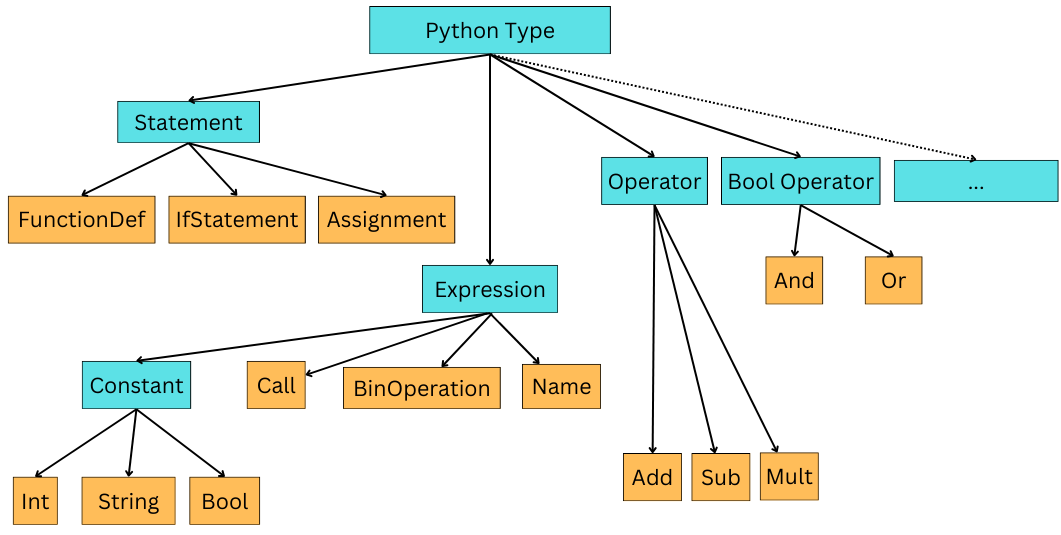
\includegraphics[scale=0.5]{img/python_hierarchy}
\end{figure}


The AST representation in Kotlin uses hierarchy of classes and interfaces.
The figure~\ref{fig:python_hierarchy} shows a subset (the whole hierarchy is much larger) of the classes (yellow boxes),
and interfaces (blue boxes).

Each class represents a node in the abstract syntax tree.
The nodes of the tree have children depending on their semantics.
For example the node Module has a list of nodes Statements representing the body of the module.
Another good example is an IfStatement, which has test Expression as a child, list of statements as the body of the
if-statement and another list of statements as the body of the else branch.

Additionally, each node implementing the Statement interface has also information about the location of the statement
in the script file - line numbers and column numbers.

\subsection{Analysis Context}\label{subsec:analysis-context}

When traversing the AST and interpreting the program, we have to keep track of all currently known variables.
We also need to store the errors and warnings generated.
We introduce the Analysis Context structure for this purpose.
In the implementation, AnalysisContext is an interface providing us with function such as getStruct, upsertStruct,
addWarning, addError and more.
There are two classes implementing this interface - GlobalAnalysisContext and FunctionAnalysisContext.

GlobalAnalysisContext is the context that keeps track of all global variables and functions and Python builtin functions
as well.
It also contains metadata about the CSV files that we read from and write to.

FunctionAnalysisContext on the other hand is created when a function is invoked.
It contains a reference to outer analysis context and a global analysis context.
It redirects the addWarning and addError function to the outer analysis context, and it also redirects the getStruct
function to the global analysis context in case that it does not know the requested variable.
This ensures that the concept of global and local variables works properly.

When the analysis is done, the global analysis context has a summarize function, which returns a summary of the analysis.

\subsection{Python structures representation}\label{subsec:python-structures-representation}

When we discussed the Analysis Context, we said that it keeps all currently active variables.
We use polymorphism to keep track of variables with dynamically resolved type.
We define the interface PythonDataStructure.
Every Python data type has to implement the PythonDataStructure interface.
The interface contains methods representing what we can do with any Python data type.
There are functions for the implementation of binary operators such as add, subtract, multiply, etc., unary operators
such as unary plus or unary minus, subscript function (the square bracket operator), the invoke function
(the parenthesis operator) and the attribute function (used for the dot notation).

All these functions return the following type:
\begin{verbatim}
   OperationResult<PythonDataStructure>
\end{verbatim}
So the operations return a PythonDataStructure, but it is wrapped inside the OperationResult.
The OperationResult is a sealed interface (meaning that all who implement the interface must be known at compile time).
There are three classes implementing the OperationResult interface: OK, Warning and Error.
OK signalizes that the operation succeeded, and it contains the result PythonDataStructure.
Warning tells us that the operation was successful but some warnings were raised during the execution.
The Warning type contains the result PythonDataStructure and a list of warnings - strings.
Last type is the Error.
It tells us that the operation failed, and it also provides a reason string.

We said that every Python data type has to implement the PythonDataStructure interface.
We would like to define abstract versions of standard Python types, meaning PythonString, PythonInt, PythonBool,
PythonNone, PythonList or PythonDict.
There are also functions (yes, a function is also a PythonDataStructure).
This includes (subset of) Python builtin functions such as \verb|print, list, len, int, or abs| as well as other
functions defined in the current scope.
Another things that also implement the PythonDataStructure are imports.
Currently, the only supported import is PandasImport, but the implementation can be easily extended by others.
The Pandas data types support is added by creating DataFrame and Series classes that also implement the PythonDataStructure
interface.

\subsection{Nondeterminism, unknown values and error recovery}\label{subsec:nondeterminism}

There are three ways in which we handle uncertainty.
The first one corresponds to the SomeString/SomeList/\ldots structures mentioned in the previous chapter.
Recall that these structures represent the knowledge of the type but the absence of the knowledge of the value.
In the implementation of Pandalyzer, this concept is represented by the fact that the values inside PythonString,
PythonList, \ldots are nullable.
In other words the PythonString(value=null) represents a string with unknown value.

The second form of uncertainty is the Nondeterministic data structure (also defined in the previous chapter).
This is uncertainty between two possible values.
In the implementation of Pandalyzer, this is represented by NondeterministicStructure with left and right
PythonDataStructure.
The NondeterministicStructure(left=PythonList([]), PythonInt(null)) represents a value that is either an empty list or a
some unknown number.
When we perform and operation on this structure, it internally performs the operation on both options and then
returns both results wrapped in a new NondeterministicStructure.

The last form of uncertainty is the UnresolvedStructure (also defined in the previous chapter).
It simply means that we do not know at all what the value is.
It happens when there is an error, and it is a part of the error recovery mechanism of the analyzer.
When we try to do an operation that is not permitted, the result of that operation is the UnresolvedStructure with
reason inside.
The reason is then added to the list of all errors.

\xxx{fork-join pattern on analysis context on if-statements}

\subsection{Dataframe and Series Representation}\label{subsec:dataframe-and-series-representation}

The Dataframe and Series representation mostly correspond to the Dataframe Structure and Series Structure defined in the
previous chapter.
The listing~\ref{lst:dataframe_definition} shows the definition of DataFrame in the Pandalyzer source code.

\begin{lstlisting}[caption=Kotlin definition of the Dataframe, label={lst:dataframe_definition}, captionpos=b]
data class DataFrame(
    val fields: MutableMap<FieldName, FieldType>?,
) : PythonDataStructure
\end{lstlisting}

The DataFrame class implements the PythonDataStructure interface since it is a type in Python.
It has a single (mutable) map, where the key type is a FieldName, which is a string.
The FieldType is an enum of all possible types that a column of a Dataframe in Pandas can have.
Also note that the map is nullable.
The DataFrame(fields=null) represents a Dataframe with unknown Dataframe Structure.

The listing~\ref{lst:series_definition} shows the definition of Series in the Pandalyzer source code.

\begin{lstlisting}[caption=Kotlin definition of the Series, label={lst:series_definition}, captionpos=b]
data class Series(
    val label: FieldName?,
    val type: FieldType?,
) : PythonDataStructure
\end{lstlisting}

The Series class also implements the PythonDataStructure interface.
The Series keeps the type information as well as the label.
Note that both the fields are nullable, meaning that it can happen that we do not know them.

Another Pandas types implemented in the Pandalyzer are SeriesGroupBy and DataframeGroupBy - the results of the groupby
operation.

\subsection{The Abstract Operations}\label{subsec:the-abstract-operations}

When implementing the abstract operations, we have to perform many check before the abstract operation itself.
We have to validate all the arguments - they can be nondeterministic, they can have null value inside, or, if they are
a compound type (list or dictionary), they can have an element that has a null value inside.

We present the idea of the implementation on an example.
The example is the rename function of a Dataframe.
It (in its simplest form) accepts an argument containing a dictionary mapping old column names to new column names.
The rename call can look as follows: \verb|df.rename({"old1": "new1", "old2": "new2"})|.

The \verb|df.rename| says that we are accessing |rename| attribute of the |df|.
The implementation of |attribute| function of DataFrame is shown in the listing~\ref{lst:dataframe_attribute}

\begin{lstlisting}[caption=Snippet of attribute function of Dataframe, label={lst:dataframe_attribute}, captionpos=b]
override fun attribute(identifier: Identifier
        ): OperationResult<PythonDataStructure> =
    when (identifier) {
        "rename" -> DataFrame_RenameFunc(this).ok()
        "merge" -> DataFrame_MergeFunc(this).ok()
        \* snip... other functions *\
        else -> fail(
            "Unknown identifier on dataframe: $identifier"
        )
    }
\end{lstlisting}

The attribute function accepts the \verb|identifier| argument and checks if it is the name of one of the known functions.
If it finds the right function, it returns the object representing the function (wrapped in an OperationResult).

Then the part \verb|rename(...)| means that we call invoke on the \\ DataFrame\_RenameFunc object.
The invoke function parses the argument, checks that it is a PythonDict, does non-deterministic split if necessary and
calls the rename function which performs the logic of the rename operation.
The invoke function is rather technical so we skip that.
Let us instead discover what the rename function of DataFrame\_RenameFunc object looks like.
%It can be seen in the listing~\ref{lst:rename_invoke}

\begin{lstlisting}[caption=The rename function of DataFrame\_RenameFunc, label={lst:rename_invoke}, captionpos=b]
private fun rename(dict: PythonDict
    ): OperationResult<PythonDataStructure> {
    if (dict.values == null) {
        return DataFrame(null)
            .withWarn("Unable to rename dataframe
                because the values of dictionary are unkown")
    }
    if (dataFrame.fields == null) {
        return DataFrame(null)
            .withWarn("Unable to rename
                dataframe with unknown structure")
    }

// check that the old values in the mapping dict are all strings
    val nonStringOldValues = dict.values
        .filterKeys { (it is PythonString).not() }.keys
    if (nonStringOldValues.isNotEmpty()) {
        return fail("The old column names
            should be strings, but were $nonStringOldValues")
    }

// check that the new values in the mapping dict are all strings
    val nonStringNewValues = dict.values
        .filterValues { (it is PythonString).not() }.values
    if (nonStringNewValues.isNotEmpty()) {
        return fail("the new column names
            should be strings, but were $nonStringNewValues")
    }

// check that the old and new values in the mapping are known
    val nullMapping = dict.values.map {
        (it.key as PythonString).value
            to (it.value as PythonString).value
    }
    if (nullMapping.any {
        it.first == null || it.second == null }){
        return DataFrame(null)
            .withWarn("Unable to resolve
            some mapping parts of rename function")
    }
    val mapping = nullMapping
        .associate { it.first!! to it.second!!}

    // check that all the old values exist in the dataframe
    val missingOldValues = mapping.keys
        .filterNot { it in dataFrame.fields }
    if (missingOldValues.isNotEmpty()) {
        return fail("The values $missingOldValues
            do not exist in the dataframe")
    }

// check that new values are not colliding with old values
    val collidingValues = mapping
        .filter { it.value in dataFrame.fields }
    if (collidingValues.isNotEmpty()) {
        val message =
            collidingValues
                .map {
            "Cannot rename a dataframe column
            ${it.key} to ${it.value} " +
            "since ${it.value} already
            exists in the dataframe"
                }
                .joinToString("\n")
        return fail(message)
    }

    // check that there are no duplicate new values
    val duplicateValues = mapping.values
        .groupBy { it }.filterValues { it.size > 1 }
    if (duplicateValues.isNotEmpty()) {
        return fail("There are duplicate new values in
            the rename function: ${duplicateValues.keys}")
    }

    return DataFrame(fields = dataFrame.fields
        .mapKeys { mapping[it.key] ?: it.key }.toMutableMap()
    ).ok()
}
\end{lstlisting}

Note that the example was altered to fit horizontally on the page.
The rename function first checks that no value needed to determine the result is null.
It also checks that both the keys and values are all strings, since that is the only accepted option for a rename
function.
The next check ensures that the keys in the dictionary have a corresponding columns in the Dataframe.
Last thing that the function checks are collisions and duplicates.
Then, new Dataframe with the new column structure is returned.
Note that we fail only if there is something wrong.
We do not fail if we do not have enough information.
Rather we return a Dataframe with unknown structure and also add a warning.

\subsection{Design Decision - Configuration file}\label{subsec:configuration-file}

When we defined the goals of the implementation, we mentioned the fact that Pandas Dataframes are usually loaded
from a CSV file.
We stated a requirement that the analyzer should not try to read the file.
The analyzer should instead receive the information about the CSV file structures from the user in some other way.
This has the advantage that the CSV files do not have to exist at all yet during the analysis as long as we know their
structure.

This, however, raises a question: How should the Pandalyzer receive the information from the user?
The following options were considered:
\begin{itemize}
    \item The user specifies the CSV structures as a command-line arguments

    This was not accepted since it is not practical for the case when the set of CSV files is bigger or the CSV files
    have many columns.

    \item The user adds the information straight to the Python code via some annotation or nop operation

    This was also rejected since the user has to make changes to the code, and it could make the code less readable.

    \item The tool will ask the user for the information once it recognizes the read\_csv function

    The problem with this approach is that it needs a lot of interaction with the user, and it complicates automatic
    execution of the analysis.

    \item The user will provide a configuration file with the CSV structures

    This approach has the advantage that it is relatively easy to specify many files that have many columns.
    Also, the configuration can be written just once in a whole project and be a part of the repository.
    So we chose this approach in the implementation.
\end{itemize}

The format of the configuration file can be best explained by an example.

\begin{lstlisting}[caption=An example configuration file, label={lst:config_example}, captionpos=b]
[file.csv]
column1 = "string"
column2 = "int"

[file2.csv]
columnA = "int"
columnB = "int"
columnC = "int"
\end{lstlisting}

As seen in the Listing~\ref{lst:config_example}, the format is inspired by a well known configuration format
TOML~\cite{toml_spec}.
We chose TOML because of its excellent readability.
However, we do not use the TOML language but only a small modified subset.
Definition of each file structure begins with a line containing the (relative or absolute) path to the file in the file
system surrounded by square brackets.
Note that this is already not a TOML, since the path to file can also contain dots or slashes which is not permitted in
TOML specification.
Following lines contain the specification of columns starting with column name, then equal sign and then the type of the
column surrounded by double quotes.

Other feature of the configuration is the regex-based file definition.
When we prepend the line containing definition of new file structure with the letter \verb|r|, the filename is
considered a regex pattern and each file matching the pattern will have the defined structure.
The idea is shown in the Listing~\ref{lst:regex_example}.

\begin{lstlisting}[caption=An example regex-based file definition, label={lst:regex_example}, captionpos=b]
r[^\d\d_file\.csv]
col = "string"
\end{lstlisting}

This means that files with names such as 01\_file.csv, 02\_file.csv, 99\_file.csv have one column of type string.

\section*{Summary}
\addcontentsline{toc}{section}{Summary}

We presented the Pandalyzer - a data manipulation code analyzer for Python and Pandas.
The tool loads the Python code, then parses it and converts it to the AST using a Python script.
Then the AST is traversed and partially interpreted.
We keep the Analysis Context with all variables, warnings and errors.
The data structures are represented by a set of classes implementing the PythonDataStructure.
The uncertainty is handled using the NondeterministicDataStructure, UnresolvedDatastructure and null values inside the
typed structures.
The Pandas structures - Dataframe and Series - correspond to the Dataframe Structure and Series Structure defined
in the previous chapter.
The operations implement a lot of checks that should prevent the user from doing many common mistakes.
The Pandalyzer also supports config file, where the user can specify the structure of the input csv files.
The planned future extensions are mentioned in the Future Work~\ref{sec:future-work} section of the Conclusion.